\documentclass[11pt]{article}

\usepackage[margin=1in]{geometry}
\usepackage{amsmath,amssymb}
\usepackage{graphicx}
\usepackage{booktabs}
\usepackage{microtype}
\usepackage[dvipsnames]{xcolor}
\usepackage{tikz}
\usetikzlibrary{arrows.meta,positioning}
\usepackage[colorlinks=true,linkcolor=RoyalBlue,citecolor=RoyalBlue,urlcolor=RoyalBlue]{hyperref}
\usepackage[capitalize,noabbrev]{cleveref}
\usepackage[round]{natbib}

\newcommand{\Jspace}{J\mbox{-}space}

\title{\bf The Workspace Survives Where the Circuit Dies:\\
Routing Is Not Computation}

\author{Siddhartha Dalal \and Vishal Misra \and Abhay Parekh}
\date{July 2026 (working note)}

\begin{document}
\maketitle

\begin{abstract}
Anthropic's J-lens finds a global workspace in production language
models: a small residual subspace carrying reusable content with a
verified causal role. What the content is, and how the workspace forms,
cannot be checked at scale. We run the lens inside Bayesian wind
tunnels, small transformers with an analytic posterior at every
position, under five preregistered predictions. Three pass: the
workspace is the hypothesis frame, its contents are the posterior's
surviving hypothesis set, and swapping its content redirects the model
to the Bayes posterior of the swapped evidence, while the uncertainty
readout riding on it is decodable and causally inert. Probing alone
locates nothing: random subspaces decode nearly as well, and never
redirect. The two failures
matter more. The workspace is written by a bank of heads, not one. And
at a loss-horizon compilation boundary the workspace survives while the
computation that fills it dies: transplanting a working writer's state
restores prediction from $0.19$ to $1.00$, and corrupting the
frame-orthogonal complement destroys prediction at every depth while
frame-specific damage is confined to the entry band. Routing substrate is not writer computation. The
separation replicates on an LSTM and a state-space model; the
frame-aligned workspace itself is the transformer's implementation, the
LSTM holds the same content in a private code, and Mamba holds it in
scan state, where a residual-stream positional lens cannot see it.
\end{abstract}

\section{Introduction}

\citet{anthropic2026workspace} report that production language models
contain a ``global workspace'': a low-dimensional subspace of the residual
stream, identified by Jacobians from internal activations to future output
logits, that is (i) read from and written to far more densely than random
directions, (ii) reused flexibly across tasks, and (iii) causally
necessary under patching. The finding is striking and the released
method is clean, but it lives where all production-scale interpretability
lives: without ground truth. What the workspace \emph{should} contain,
which components \emph{should} write it, and what its formation
\emph{should} look like are all unavailable at scale. The paper's own open
question is the mechanism: what decides what enters the workspace, and how
does it form?

Bayesian wind tunnels~\citep{agarwal2026windtunnel} were built for exactly
this epistemic situation. In the bijection wind tunnel, a 2.7M-parameter
transformer learns in-context inversion of a random bijection; the
analytic posterior at every position is known in closed form, the trained
model is functionally Bayesian (entropy calibration within $0.007$ bits of
the posterior), and the internal mechanism is characterized: a Layer-0
hypothesis frame, elimination through middle layers, refinement late, with
a derived formation account from advantage-based routing under normalized
competition~\citep{agarwal2026gradient}. If the global workspace is a real
object rather than an artifact of the lens, running the J-lens in a wind
tunnel should find it, and should find it \emph{equal to} the hypothesis
frame, an identification that grounds the workspace in a setting where
its contents can be checked against Bayes and supplies the formation
mechanism the production-scale paper lacks.

The distinction matters. In production
models, the J-lens identifies a causal subspace but cannot say what
semantic object it has recovered. In the wind tunnel, where the analytic
posterior is known, we can check this directly: the \Jspace{} is not
merely workspace-\emph{like}; it is the hypothesis frame carrying the
surviving posterior support. What follows is not a validation of the
production finding but an identification result in miniature.

We preregistered five predictions (P1--P5) with quantitative thresholds
before running anything, including two designed to be falsifiable in
specific directions. Three passed. The two failures are the most
informative results in the note. The experiment could have failed in
three qualitatively different ways: the \Jspace{} could have aligned
with generic token/unembedding geometry rather than the hypothesis frame
(the random-initialization and MLP controls test this); it could have
decoded hypothesis identity without carrying posterior support (the P3
probes and per-hypothesis decay curves test this); or it could have
patched causally without matching the Bayes posterior of the injected
evidence (the P4 swaps, scored against the donor's analytic posterior,
test this). The controls and swaps distinguish these cases.

\paragraph{Summary of findings.}
\begin{enumerate}
  \item \textbf{Identity (P1, pass).} The \Jspace{} at the
  embedding/block-0 band coincides with the hypothesis frame in
  token-identity coordinates at $4.8$--$6.8\times$ a matched-dimension
  random-subspace null, robust to the Jacobian horizon; a
  random-initialization control and a trained, parameter-matched MLP
  control both sit at the null, so the alignment is learned structure,
  not unembedding geometry.
  \item \textbf{Writers (P2, fail as preregistered; sharper replacement
  result).} No single head dominates workspace writing. Instead the nine
  indispensable heads (the full Layer-0 bank plus three Layer-1 heads)
  separate from the remaining 27 with \emph{zero overlap} in absolute
  frame-projected write norm.
  \item \textbf{Contents (P3, pass).} Per-hypothesis probes on \Jspace{}
  coordinates decode eliminated-vs-surviving status at $97.7\%$
  ($r{=}24$) and $99.8\%$ ($r{=}32$) balanced accuracy; the rank
  dependence itself confirms that the workspace dimension is the
  hypothesis count.
  \item \textbf{Causal asymmetry (P4, pass).} Swapping \Jspace{} content
  between evidence-matched runs redirects the model's posterior to the
  donor's Bayes posterior ($+2.9$ bits for the $r{=}16$ \Jspace{};
  $+8.2$ bits, the full-residual ceiling, for the frame). Ablating the
  entropy-readout axis, which is perfectly linearly decodable
  ($R^2{=}1.00$), changes calibration by $-0.001$ bits: readable but
  causally inert. The frame--precision dissociation of
  \citet{agarwal2026unified} replicates inside the wind tunnel.
  \item \textbf{The horizon boundary (P5, preregistered reverse finding).}
  In $K{=}5$ loss-horizon models the calibration cliff replicates
  ($0.005$--$0.11$ bits inside the horizon; $1.3$--$1.8$ bits past it),
  but the workspace does \emph{not} collapse: frame overlap stays at
  $4.8\times$ null past the boundary while the last-layer next-token
  computation dies ($0.77 \to 0.19$ decode). The compilation boundary
  lives in the writers, not the workspace.
  \item \textbf{Cross-architecture (exploratory).} The separation
  principle and the frame--precision dissociation replicate on an LSTM
  (three seeds) and a Mamba-style SSM; the frame-aligned workspace
  itself does not. The LSTM holds the same causally swappable content
  in a private code; Mamba holds it in scan state, unreachable by
  positional patching but causally confirmed by state-level
  intervention (\cref{sec:crossarch}).
\end{enumerate}

\begin{table}[t]
\centering
\resizebox{\textwidth}{!}{%
\begin{tabular}{@{}llll@{}}
\toprule
 & \textbf{Preregistered claim} & \textbf{Threshold} & \textbf{Outcome} \\
\midrule
P1 & \Jspace{} $=$ frame subspace & $\ge 3\times$ null; decode $\ge 90\%$ &
  \textbf{Pass} ($4.8$--$6.8\times$; controls at null) \\
P2 & Frame head dominates writing & $\ge 2\times$ every other head &
  \textbf{Fail} $\to$ 9-head bank, zero-overlap dichotomy \\
P3 & Contents $=$ surviving set & $\ge 95\%$ (balanced) &
  \textbf{Pass} ($97.7\%$ at $r{=}24$; $99.8\%$ at $r{=}32$) \\
P4 & Swap redirects; entropy axis inert & $\ge 1$ bit; calibration intact &
  \textbf{Pass} ($+2.9$ bits; $\Delta$MAE $-0.001$) \\
P5 & Workspace collapses past horizon & post-horizon $\le$ null &
  \textbf{Reverse} ($4.8\times$ null; computation $0.77 \to 0.19$) \\
\bottomrule
\end{tabular}}
\caption{Preregistration scorecard. Full thresholds, per-cell grids, and
deviations are in the repository.}
\label{tab:scorecard}
\end{table}

\section{Setup}

\paragraph{Models.} The primary model is the bijection wind-tunnel
transformer of \citet{agarwal2026windtunnel}: 6 layers, 6 heads,
$d{=}192$, 2.69M parameters, vocabulary $2V$ with keys $0..V{-}1$ and
values $V..2V{-}1$ ($V{=}20$), trained on sequences
$[k_1, v_1, \dots, k_L]$ with every key position supervised to predict
the upcoming value. The trained model's entropy calibration MAE is
$0.0067$ bits. Controls: the same architecture at random initialization,
and a parameter-matched (2.68M) attention-free residual MLP trained to
its plateau ($1.107$ bits; it cannot bind in context, which is the
point). For P5 we use the $K{=}5$ loss-horizon recurrence models of the
companion manuscript~\citep{misra2026nature} (three seeds; modular linear
recurrence $x_{t+1} = ax_t + b \bmod 17$, loss restricted to positions
$1..5$ of 16) and a full-horizon control.

\paragraph{J-lens.} We follow the released
operationalization~\citep{anthropic2026jlens} with deviations recorded in
the repository's \texttt{DEVIATIONS.md}, the substantive one being
resolution: their estimator averages the Jacobian over source positions;
the wind tunnel's mechanism is position-specific, so we keep per-$(\ell,
i)$ resolution. For residual activation $x$ at layer $\ell$, position
$i$, the \Jspace{} is the top-$r$ right singular subspace of the stacked
rows $\{\partial \mathrm{logits}[p', v] / \partial x : v \in
\text{hypotheses},\ p' > i\}$ over 256--512 held-out sequences,
accumulated as a Gram matrix (the sweep over all layers and positions
costs seconds; the entire study used ${\sim}2$ GPU-hours against a
60--120 hour budget). This is not circular: restricting the
cotangent dimensions to the hypothesis tokens does not aim the lens at
the frame, because the hypothesis tokens \emph{are} the model's output
vocabulary (only value positions are supervised), so the restriction is
``all potential outputs,'' which is the released lens's own definition,
not a frame-specific choice. Subspace stability across disjoint batches is
$0.95$ mean projection overlap (gate G0). Overlap ratios are quoted
against the null mean; against the null's 99th percentile the headline
$6.1\times$ becomes $4.9\times$. The results are unchanged under the
released estimator's own cotangent aggregation (summed over future
positions: $5.9/3.6/1.8$ versus $6.1/3.9/1.9$ across the carrying
band), so nothing rests on our per-position refinement. The comparison frame is the
span of the $V$ hypothesis-token directions as Layer-0 attention sees
them (embedding mode), with the Layer-0 head-pullback variants (key-read,
OV-write) reported alongside.

\begin{figure}[t]
  \centering
  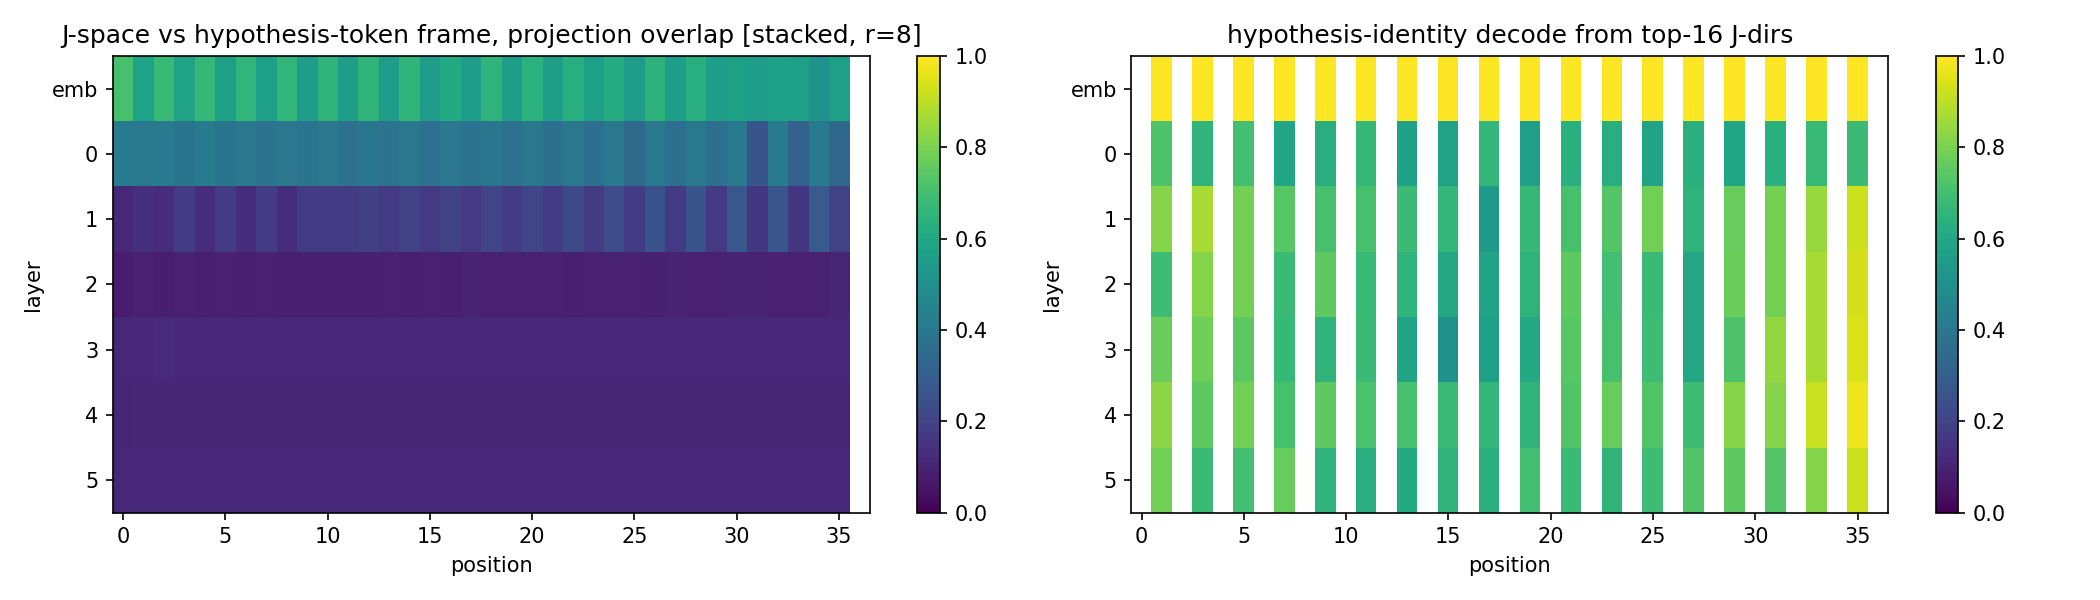
\includegraphics[width=\textwidth]{figures/phase1_heatmaps.png}
  \caption{\textbf{P1: the \Jspace{} is the hypothesis frame.} Left:
  projection overlap between the per-$(\ell, i)$ \Jspace{} ($r{=}8$) and
  the hypothesis-token frame across layers (rows) and positions
  (columns); the carrying band is the embedding/block-0 residual. Right:
  hypothesis-identity decoding from the top-16 \Jspace{} directions.
  Late-layer cells are structurally degenerate for strictly-future
  targets (causality), so workspace claims are inherently early/mid-layer
  claims.}
  \label{fig:p1}
\end{figure}

\begin{figure}[t]
  \centering
  \resizebox{\textwidth}{!}{%
  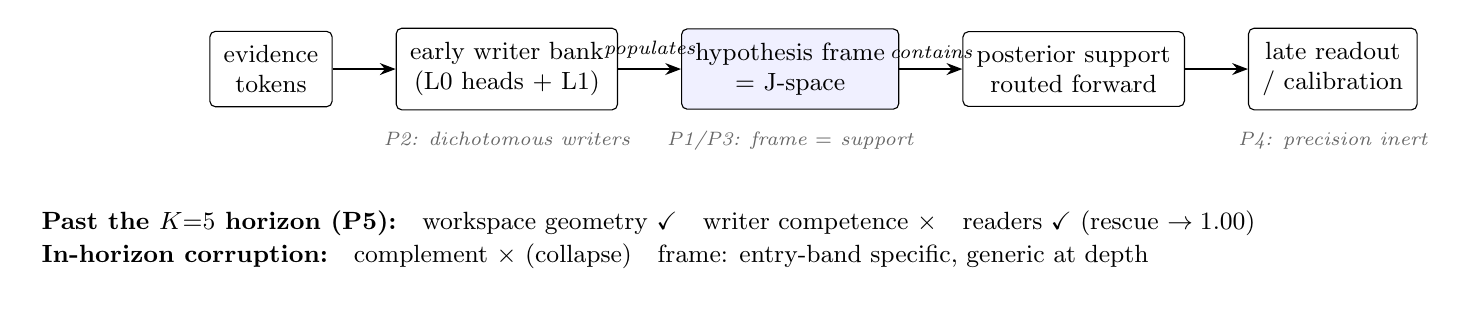
\begin{tikzpicture}[
      node distance=4mm and 8mm,
      box/.style={draw, rounded corners=2pt, align=center,
                  minimum height=8mm, inner sep=5pt, font=\small},
      lbl/.style={font=\scriptsize\itshape, text=black!60},
      arr/.style={-{Stealth[length=2mm]}, thick}]
    \node[box] (ev) {evidence\\tokens};
    \node[box, right=of ev] (wr) {early writer bank\\(L0 heads $+$ L1)};
    \node[box, right=of wr, fill=blue!6] (ws) {hypothesis frame\\$=$ \Jspace{}};
    \node[box, right=of ws] (rt) {posterior support\\routed forward};
    \node[box, right=of rt] (rd) {late readout\\/ calibration};
    \draw[arr] (ev) -- (wr);
    \draw[arr] (wr) -- node[above, font=\scriptsize\itshape] {populates} (ws);
    \draw[arr] (ws) -- node[above, font=\scriptsize\itshape] {contains} (rt);
    \draw[arr] (rt) -- (rd);
    \node[lbl, below=1.5mm of wr] {P2: dichotomous writers};
    \node[lbl, below=1.5mm of ws] {P1/P3: frame $=$ support};
    \node[lbl, below=1.5mm of rd] {P4: precision inert};
    \node[box, below=11mm of ws, xshift=-18mm, draw=none, align=left,
          font=\small] (ph) {\textbf{Past the $K{=}5$ horizon (P5):}\quad
      workspace geometry \checkmark\quad
      writer competence $\times$\quad
      readers \checkmark\ (rescue $\to 1.00$)\\[1pt]
      \textbf{In-horizon corruption:}\quad
      complement $\times$ (collapse)\quad
      frame: entry-band specific, generic at depth};
  \end{tikzpicture}}
  \caption{The workspace pipeline as identified in the wind tunnel, with
  the phase that tests each stage, and the P5 dissociation: past the
  compilation boundary only the writers fail; in-horizon corruption
  places the in-flight computation in the frame's complement.}
  \label{fig:schematic}
\end{figure}

\section{Results}

\subsection{P1: the workspace is the frame, in token coordinates}

At the embedding/block-0 band the \Jspace{} overlaps the
hypothesis-token frame at $4.8\times$ ($r{=}4$), $6.1\times$ ($r{=}8$),
and $6.8\times$ ($r{=}16$) the matched random-subspace null
(\cref{fig:p1}), identically for both Jacobian reductions and essentially
unchanged when targets are restricted to ${\ge}2$ positions ahead (the
unembedding-geometry robustness check: $4.7/5.9/6.6$). The two controls
are decisive (\cref{tab:controls}): the same architecture at random
initialization gives $1.1$--$1.2\times$, and the trained MLP control
gives $0.9$--$1.2\times$. The alignment is learned, and it is not the
tied unembedding.

\begin{table}[h]
\centering
\small
\begin{tabular}{@{}lll@{}}
\toprule
\textbf{Condition} & \textbf{\Jspace{}/frame overlap} & \textbf{Rules out} \\
\midrule
trained transformer & $4.8$--$6.8\times$ null & --- \\
random-init transformer & $1.1$--$1.2\times$ & architecture / unembedding geometry \\
trained MLP (2.68M, plateaued) & $0.9$--$1.2\times$ & training without in-context binding \\
trained, untied embeddings & $1.5$--$1.9\times$ & frame coordinates without weight tying \\
\bottomrule
\end{tabular}
\caption{P1 controls. The frame alignment requires \emph{trained
attention}: neither the architecture's geometry nor training per se
produces it.}
\label{tab:controls}
\end{table}

Two further controls, both referee-requested, bound the identity
claim. An \emph{untied-embedding} transformer trained to calibration
($0.017$ bits) shows frame alignment of only $1.5$--$1.9\times$ at
every layer: the strong token-frame coordinates of the production
model are in substantial part a product of weight tying. And across
training seeds the magnitude varies widely ($2.3$--$6.1\times$ at the
embedding band; all above null, not all above the $3\times$ gate), with
causal swap margins scaling accordingly ($+1.0$ to $+8.2$ bits). What
is seed- and tying-invariant is the structure underneath: contents
decode at $1.000$ on every seed, the entropy axis is causally inert on
every seed, and projecting out the frame destroys calibration on every
seed ($+1.05$ to $+1.06$ bits). The identification should therefore be
read at two levels: the separation structure is invariant; the degree
of externalization into token coordinates is contingent, on tying, on
seed, and (\cref{sec:crossarch}) on architecture.

Two refinements against the strict preregistration. First, the frame
operationalization that carries the identity is the \emph{token-identity}
frame (embedding directions of the hypothesis tokens); the Layer-0
head-pullback variants pass only at low rank (key-read $3.5$--$4.6\times$
at $r{=}4$), i.e.\ the frame head reads the \emph{leading} \Jspace{}
directions but does not exhaust the workspace. Second, the decoding half
of P1 (hypothesis identity from top-$k$ \Jspace{} directions, $100\%$)
is satisfied by the random-init control as well (token identity is
linearly present in any embedding), so P1's evidential weight rests
entirely on the trained-vs-control overlap contrast, which is $5$--$6\times$.

\subsection{P2: no dominant writer, but a clean dichotomy}

\begin{figure}[t]
  \centering
  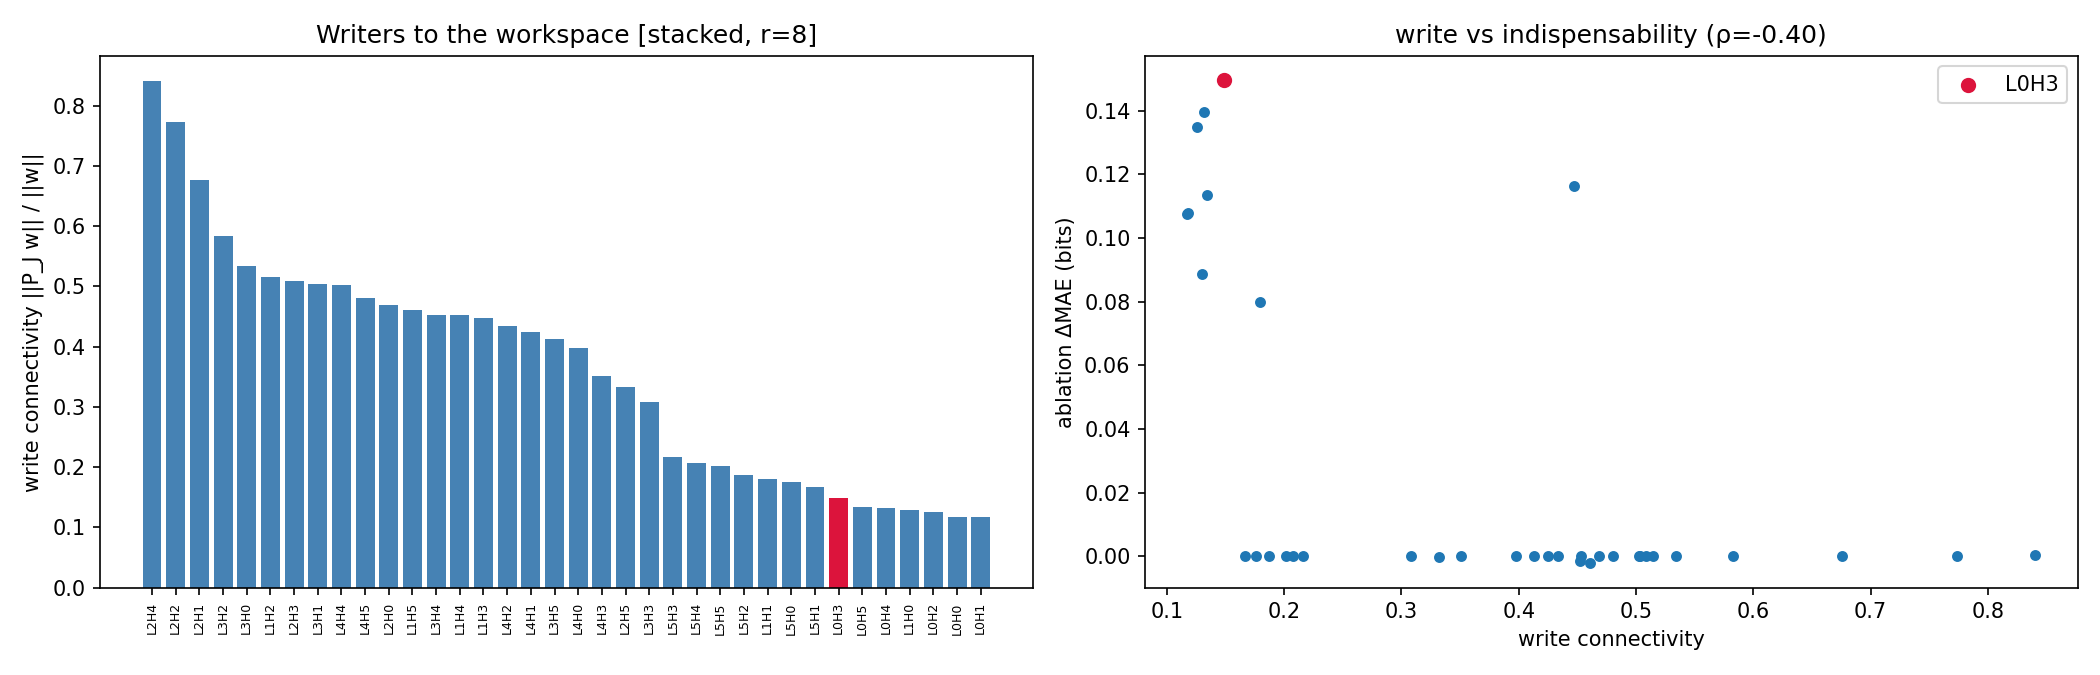
\includegraphics[width=\textwidth]{figures/phase2_writers.png}
  \caption{\textbf{P2: workspace writing is distributed but dichotomous.}
  Left: per-head write connectivity (ratio form); the metric is dominated
  by near-dead heads with tiny frame-aligned writes, which is why the
  preregistered ratio gate is the wrong metric. Right: write connectivity
  vs.\ ablation indispensability ($\Delta$MAE).}
  \label{fig:p2}
\end{figure}

The preregistered prediction, that the Layer-0 hypothesis-frame head
writes the workspace at ${\ge}2\times$ every other head, fails. It
fails at the premise: on this checkpoint \emph{indispensability itself is
distributed}. Ablating any of the six Layer-0 heads degrades calibration
by $0.11$--$0.15$ bits ($20$--$25\times$ baseline), with three Layer-1
heads close behind; there is no single uniquely destructive frame head.

This is in apparent tension with the single-frame-head claim of
\citet{agarwal2026windtunnel}, so we ran the reconciliation: the same
ablation protocol on a paper-grade retrain of Paper~I's task variant
(shared vocabulary, explicit query token; calibration $0.017$ bits).
There the claim replicates: one Layer-0 head stands out at $2.7\times$
the second, with a single head above half the top effect. The
production variant (no query token; every key position is a readout
site) instead distributes indispensability across the full Layer-0
bank. Writer
concentration tracks readout demand: one query site, one binding head;
a readout site at every position, a bank. The single-head claim is
variant-true, not architecture-general, and the two results are one
phenomenon seen at two supervision geometries.

The replacement result is sharper than the prediction it replaces.
Ranking heads by \emph{absolute frame-projected write norm}
$\lVert P_F\, w_h \rVert$, the nine indispensable heads (all of Layer 0
plus L1H0/H1/H3) separate from the remaining 27 with zero overlap:
minimum $2.06$ among the indispensable, maximum $0.75$ among the rest.
Writer magnitude into the workspace \emph{is} indispensability, as a
dichotomy (Spearman $\rho = 0.47$, $p = 0.004$ on the continuous
ranking; the within-group ordering carries no signal). The dichotomy
\emph{property} replicates on two further training seeds (clean
zero-overlap separation on both), while the writer-set composition does
not: the replication seeds recruit larger banks reaching into blocks 2
and 3. Which heads write is contingent; that writers separate cleanly
from non-writers is not. A methodological
caution for the production-scale analysis falls out of the failure: the
scale-free ratio $\lVert P_J w \rVert / \lVert w \rVert$ is gamed by
near-dead heads whose tiny writes happen to point at the workspace
(ratio-form $\rho = -0.40$ with indispensability, wrong sign); write
connectivity should be measured in absolute projected norm.

\subsection{P3 + P4: contents carry the posterior support; the model
uses the content, not the precision readout}

\begin{figure}[t]
  \centering
  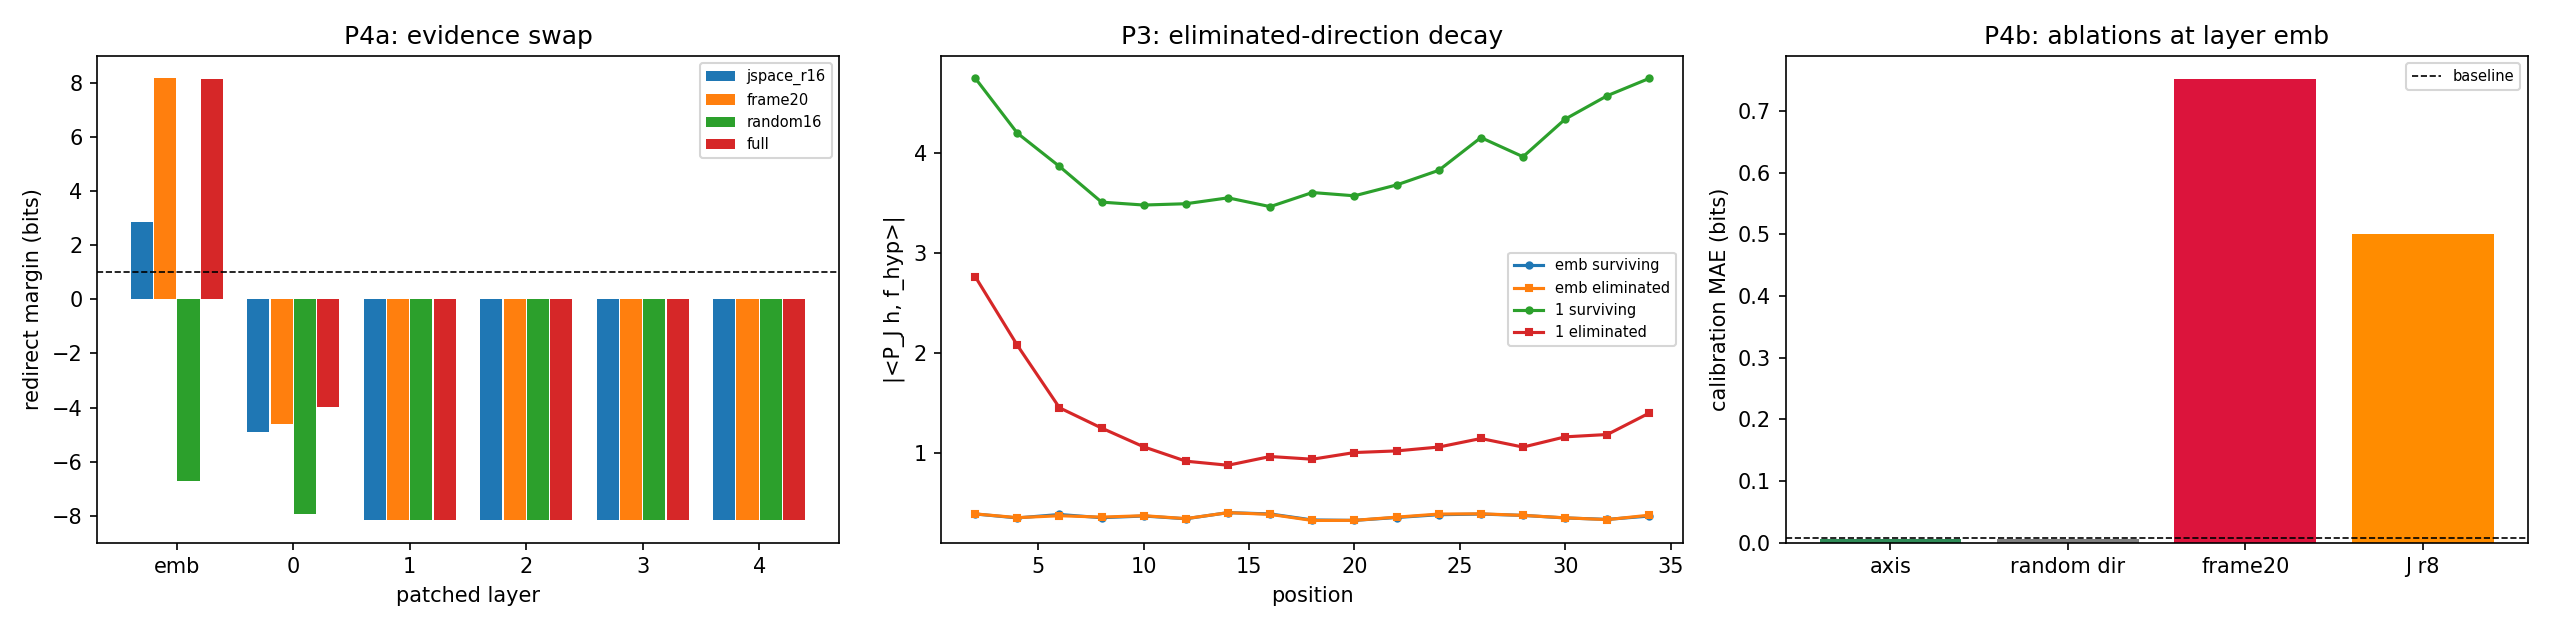
\includegraphics[width=\textwidth]{figures/phase3_causality.png}
  \caption{\textbf{P4: causal structure of the workspace.} Left:
  evidence-swap redirect margins by patched layer; the frame swap at the
  embedding equals the full-residual ceiling, the random-subspace control
  never redirects, and the injection window closes after layer 1. Center:
  eliminated-hypothesis directions decay in \Jspace{}-projected residual
  norm as elimination proceeds. Right: ablations; the entropy axis is
  causally inert, the frame is not.}
  \label{fig:p3}
\end{figure}

\paragraph{Contents (P3).} Per-hypothesis logistic probes on \Jspace{}
coordinates decode eliminated-vs-surviving status at $90.0\%$ ($r{=}16$),
$94.8\%$ ($r{=}20$), $97.7\%$ ($r{=}24$), $99.8\%$ ($r{=}32$) balanced
accuracy (full-residual ceiling $100\%$). The monotone rank dependence
crosses the preregistered $95\%$ exactly as the probe rank passes the
hypothesis count $V{=}20$. But a referee control cuts the probe
evidence down to size: random rank-matched subspaces decode at $0.96$
($r{=}24$) and $0.99$ ($r{=}32$), nearly matching the \Jspace{}.
Decodable information is promiscuous in the residual stream, so the
probe form of P3 does not locate content; it shows only that the
\Jspace{} carries what most fat subspaces also carry. This is our own
readable-is-not-used caution applied to ourselves, and it moves the
content-location claim entirely onto the causal test below, where the
discrimination is total: the \Jspace{} swap redirects ($+6.5$ bits at
matched rank $r{=}20$) and no random subspace ever does (mean $-11.5$,
maximum $-10.9$ over 100 draws). (Preregistration note: the eliminated base rate approaches $0.9$ late
in the sequence, so raw accuracy is uninformative and the gate was
evaluated with balanced accuracy.)

\paragraph{Causal asymmetry (P4).} We build evidence-matched donor pairs
(identical key order, independent permutations) and patch the \Jspace{}
component of the evidence region with the donor's. At the embedding, the
$r{=}16$ \Jspace{} swap redirects the model's posterior toward the
\emph{donor's} Bayes posterior by $+2.9$ bits (margin over the original
posterior, 256 pairs), and $+6.5$ bits at the rank-matched $r{=}20$;
the 20-dimensional frame swap redirects by
$+8.2$ bits, indistinguishable from patching the entire residual;
random matched-dimension subspaces never redirect (mean $-11.5$,
maximum $-10.9$ over 100 draws). Content routed
through the workspace is what the model treats as evidence.

The dissociation half: the entropy-readout axis (fit by ridge
regression; $R^2 = 1.00$, perfectly linearly decodable) changes
calibration by $-0.001$ bits when projected out. Projecting out the frame
costs $+0.75$ bits. Being readable and being used are different
properties, measured causally --- and the lens agrees: the entropy
axis's projection onto the top J-directions is at or below the
random-direction baseline at every layer, so the use-weighted subspace
excludes what the ablation shows to be inert; the frame--precision boundary result of
\citet{agarwal2026unified} replicates in a 2.7M-parameter model. This
also discharges a standing question from our own backlog: probes on the
$(a,b)$-style readout directions detect real structure, and that
structure can still be causally epiphenomenal. The precise statement: the workspace \emph{carries posterior
support}; precision is readable off it but not necessarily used.

\paragraph{A mechanistic bonus.} The swap experiment doubles as a causal
map of \emph{when} evidence enters the readout pathway: patches at block
outputs ${\ge}1$ have no effect at all (margins pinned at the unpatched
baseline, for every basis including the full residual). The injection
window closes after layer 1, exactly where P2 found every indispensable
writer. Two independent methods, one localization.

\subsection{P5: the reverse finding at the horizon boundary}

\begin{figure}[t]
  \centering
  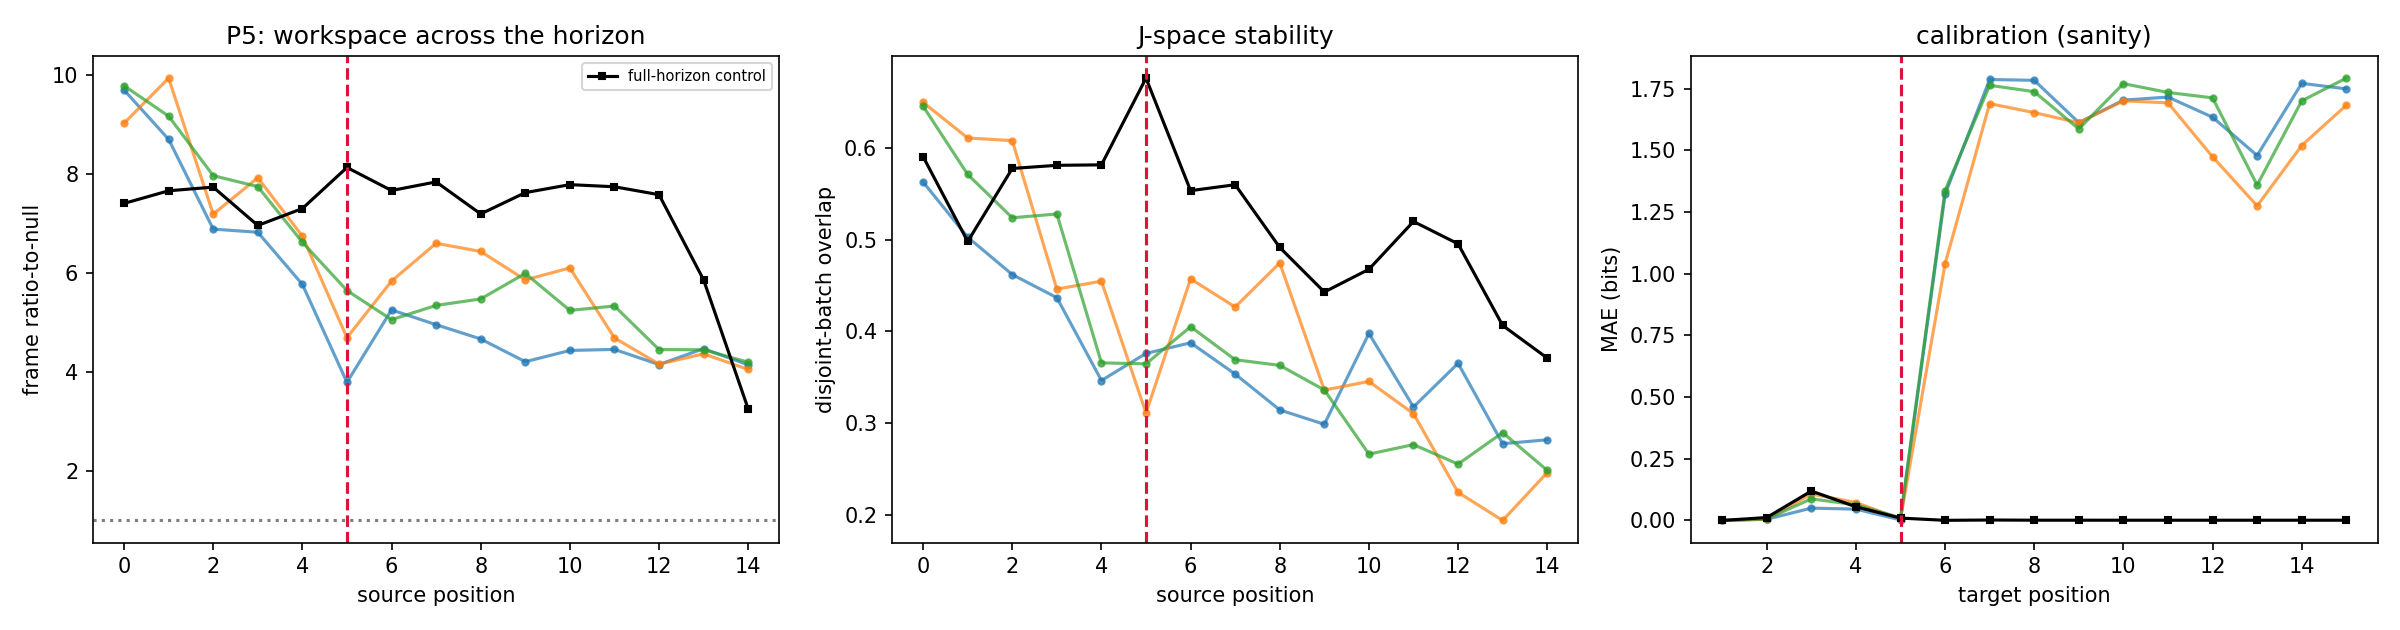
\includegraphics[width=\textwidth]{figures/phase4_horizon.png}
  \caption{\textbf{P5 reverses: the workspace survives the compilation
  boundary.} Left: frame overlap ratio-to-null by source position for
  three $K{=}5$ loss-horizon seeds (colors) and the full-horizon control
  (black); the dashed line marks the horizon. The preregistered collapse
  to null does not occur. Center: \Jspace{} stability. Right: the
  calibration cliff replicates exactly.}
  \label{fig:p5}
\end{figure}

The $K{=}5$ loss-horizon models replicate the companion manuscript's
compilation cliff precisely: calibration MAE is $0.005$--$0.11$ bits at
trained positions and $1.3$--$1.8$ bits past them, against
$0.001$ everywhere for the full-horizon control. The preregistered
prediction was that the workspace tracks the cliff: well-formed at
positions ${\le}5$, degrading to null past the boundary. The
preregistration also stated that the reverse outcome ``must be reported
if found.'' It was found (\cref{fig:p5}).

Past the horizon the frame-aligned \Jspace{} persists at $4.8\times$ null
(a decline from $6.5\times$ in-horizon, but nowhere near the
${\le}1.5\times$ collapse gate; two independent full-horizon control
seeds hold $6.7$--$7.7$ in-horizon and $6.7$--$7.1$ past it). What collapses is the
\emph{writer computation}: decoding the (deterministic) next token from
\Jspace{} coordinates at the last layer succeeds at $0.77$ inside the
horizon and falls to $0.19$ past it, while the control holds $1.00$
everywhere. The dissociation is exact: geometry global, writer computation
positional.

We read this as the strongest bridge result between the two papers. The
loss-horizon wall of \citet{misra2026nature} is real and replicates at
the circuit level. But the wall is in the \emph{writers}, the
positionally compiled machinery that fills the workspace with calibrated
content, not in the workspace itself. Conversely, the flexibility
Anthropic attributes to the workspace is a property of the routing
substrate and does not, by itself, buy generalization past a compilation
boundary: a model can carry a perfectly good workspace into positions
where nothing knows how to write to it.

\paragraph{Horizon rescue by writer patching.} The dissociation admits a
direct causal test: if the boundary lives in the writers and not in
what follows them, then handing a post-horizon position the state an
in-horizon writer would have produced should rescue the prediction.
Modular orbits make the required state-matching exact: the donor
sequence is the test sequence's orbit started six steps later, so donor
position $p$ carries the recurrence state of test position
$p{+}6$. We transplant the donor's residual at in-horizon positions
$2$--$4$ into post-horizon positions $8$--$10$. The rescue is complete
and monotone in patch depth: post-horizon accuracy goes from $0.19$
unpatched to $0.78$ (block 1), $0.98$ (block 2), and $1.00$ (block 3),
across all three seeds, while the full-horizon control is unharmed by
every patch condition. (The writer span here extends through block 3;
in the bijection model the injection window closed after layer 1. These
are different tasks with different write depths; the modular-inverse
computation is deeper than key--value binding.) The readers, everything
downstream of block 3 at that position, are position-general; given a correctly written state
they finish the computation perfectly, anywhere. Two controls sharpen
this. Transplanting only the frame-subspace component does \emph{not}
rescue ($0.21$, indistinguishable from a random-subspace transplant at
$0.24$): mid-stream, the in-flight $(a,b)$ computation lives in the
residual complement of the token frame, rotating into frame coordinates
only late. The corruption sweep below sharpens this: in the recurrence
model the frame's causal role is confined to the entry band, and the
in-flight and readout computation live in the complement. The apparent
tension with P4 is a difference between models and bands, not a
contradiction: in the bijection model the frame swap at the embedding
is the full-residual ceiling; here, past entry, the frame carries
nothing the computation uses. And patching at the
embedding does nothing ($0.20$) because the matched states share their
input token; everything the donor contributes is computed structure from
the writer layers. The compilation boundary is now causally localized:
writers (blocks 0--3 at the position) are broken past the horizon,
readers are not.

\paragraph{Writer corruption: the converse.} The loop closes from the
other direction, with a referee-requested control that changed our
reading. At \emph{in}-horizon positions, where everything works, we
corrupt the residual with norm-preserving random orthogonal rotations
at every block (1--5), in four conditions: the full residual, the
frame's orthogonal complement, the frame itself, and a random subspace
of the frame's dimension. Complement rotation collapses prediction at
every depth ($1.00 \to 0.05$--$0.36$; chance $0.06$); frame rotation
spares it at blocks 3--5 ($0.98$--$1.00$), but so does the
dimension-matched random rotation ($1.00$ everywhere), so sparing at
depth is a statement about dimension, not about the frame. The
frame-specific signal is at the entry band: at block 1, frame rotation
damages prediction ($0.38$--$0.54$) while the random matched-dimension
rotation does nothing ($1.00$), across all three seeds and the
control. The frame is causally specific where evidence enters, fades
to generic by block 3 (the same migration the rescue's depth profile
shows), and the complement carries the in-flight computation
throughout. Every condition is norm-matched; the subspace-specific
causal discrimination lives in the swap and rescue contrasts, which
are dimension-matched by construction.

\paragraph{Why the workspace must survive.} The
reverse finding is a structural consequence of weight sharing. The objects that define the workspace geometry, the token
embeddings and the QK/OV maps, are position-independent by
construction; position enters only through how those shared weights are
\emph{used}, via content routed by attention. Gradient descent under a
positional loss mask can therefore compile position-dependence only into
the computation routed through the shared weights, never into the
weights themselves: the geometry is global because nothing in the
parameterization can make it local. ``Geometry global, writer computation
positional'' is then the expected signature of positional compilation in
any weight-shared architecture, which is the thesis of
\citet{misra2026nature}, now visible through the lens. (And yes, this is
``just weight sharing''; that is the point.)

\paragraph{Dose--response.} The checkpoint family includes runs trained
with sparse post-horizon supervision (\texttt{extra\_loss\_density}
$\in \{1\%, 5\%, 25\%\}$ of post-horizon positions receiving loss),
which convert the binary reverse finding into a graded law. Across
densities $0\% \to 1\% \to 5\% \to 25\%$ (three seeds each): post-horizon
calibration MAE $1.64 \to 0.54 \to 0.014 \to 0.005$ bits and last-layer
decode $0.19 \to 0.68 \to 1.00 \to 1.00$, while the workspace overlap
ratio stays high throughout ($4.8 \to 4.8 \to 7.6 \to 7.4\times$ null).
Supervision density is the variable, writer competence is what it buys,
and the workspace is the thing it does not need to buy: even $1\%$
post-horizon supervision recovers most writer function against an
already-present substrate.

\subsection{Formation dynamics}

\begin{figure}[t]
  \centering
  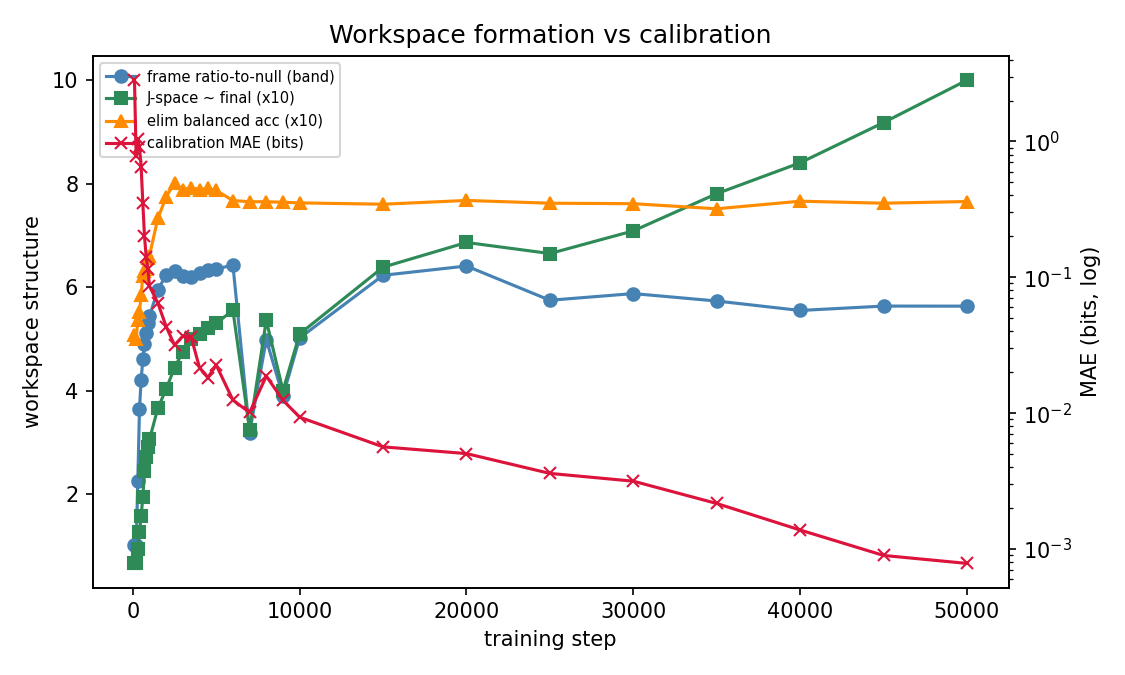
\includegraphics[width=0.62\textwidth]{figures/phase5_dynamics.png}
  \caption{\textbf{Workspace before precision} (dense-checkpoint
  retrain, steps 100--50k, log-scale MAE). The frame ratio crosses the
  P1 threshold by step 400 and plateaus by step ${\sim}2{,}500$;
  calibration MAE improves another ${\sim}40\times$ after the frame is
  in place.}
  \label{fig:dyn}
\end{figure}

A retrain with dense early checkpoints (same architecture, data
distribution, and hyperparameters, reimplemented single-GPU from the
production trainer; checkpoints every 100 steps from step 100) makes
the formation curve visible end to end (\cref{fig:dyn}). The retrain
converges somewhat further than the production checkpoint ($0.0008$ vs
$0.0067$ bits final MAE, plausibly a distributed-vs-single-GPU trainer
difference); the formation \emph{ordering}, which is the claim, is
unaffected. The frame rises
fast and first: overlap with the frame subspace is $2.3\times$ null at
step 300, crosses the P1 threshold ($3\times$) by step 400, and plateaus
near $6\times$ by step 2{,}500, at which point calibration MAE is still
$0.03$ bits and proceeds to improve another ${\sim}40\times$ (to
$0.0008$ bits) over the remaining 47k steps with the frame ratio flat.
Elimination decoding saturates on the same early schedule (0.54 at step
300, 0.79 by step 3k). The production run's checkpoints (10k--50k)
show the same plateau from above: already $3.7\times$ at its first
checkpoint, converged to the final workspace by 30k. This is the
ordering the frame--precision dissociation predicts: build the frame,
then sharpen the numbers in it.

\begin{figure}[t]
  \centering
  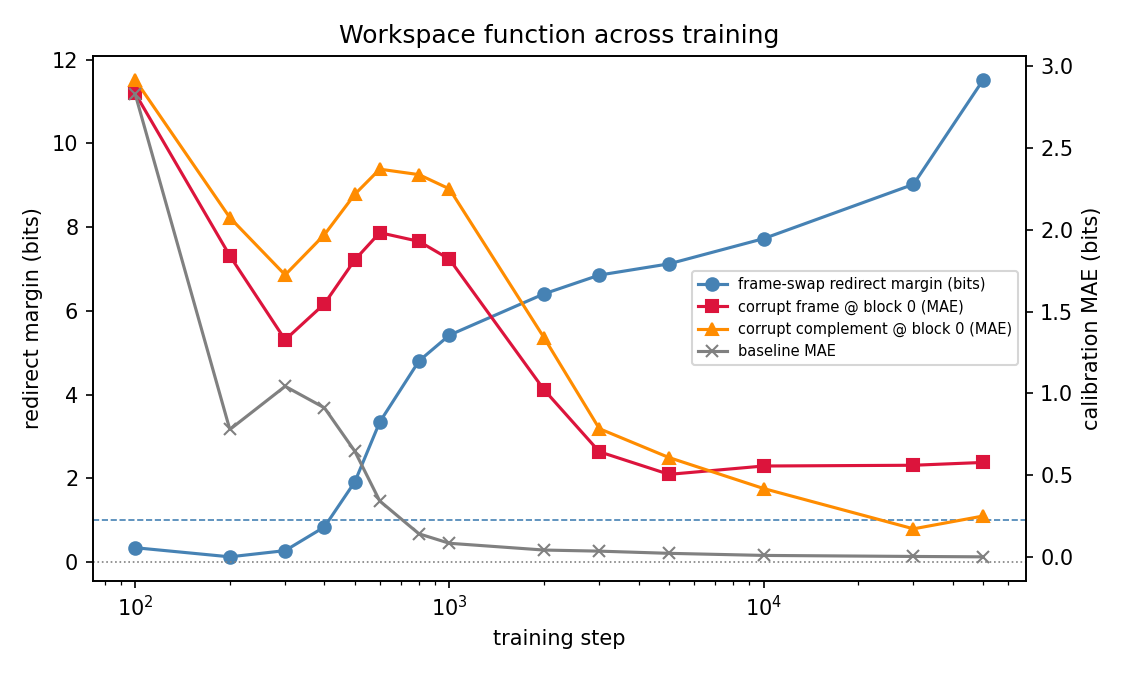
\includegraphics[width=0.62\textwidth]{figures/phase8_midtraining.png}
  \caption{\textbf{The early workspace already does causal work.}
  Per-checkpoint P4 frame-swap redirect margin (left axis) against
  calibration under frame/complement corruption at block 0 (right axis,
  log-x). The margin crosses the $+1$-bit causal threshold between steps
  400--500, as the frame crosses the P1 threshold, and grows
  monotonically thereafter.}
  \label{fig:midtraining}
\end{figure}

\paragraph{The early workspace is causally functional.} Formation and
causation sit on one x-axis in \cref{fig:midtraining}: rerunning the P4
evidence-matched frame swap at every dense checkpoint, the redirect
margin crosses the $+1$-bit success threshold between steps 400 and 500
($+0.84 \to +1.92$ bits), the same steps at which the frame crosses the
P1 overlap threshold, while calibration is still $0.65$ bits, three
orders of magnitude from converged. The margin then grows monotonically
with training ($+3.4$ at step 600, $+5.4$ at 1k, $+11.5$ at 50k).
Norm-preserving corruption at block 0 damages calibration from the
first functional checkpoint (metrics follow the task: accuracy on the
recurrence task, where the target is deterministic; calibration MAE
here, where it is a posterior), and its structure sharpens with training:
early, frame- and complement-rotation hurt about equally; by step 30k
frame-rotation is $2.3\times$ more destructive ($+0.58$ vs $+0.25$
bits), the load consolidating into the frame coordinates at the
injection band, consistent with P4's frame-ablation result. Two migration axes, one
object. Across depth within a
forward pass, content moves frame $\to$ complement $\to$ frame; across
training time, load consolidates into the frame at the injection band. The
formation story is therefore causal end to end: the workspace forms by
step ${\sim}400$, becomes causally functional as soon as it forms, and
the remaining 47k steps buy writer precision inside a
substrate that already works.

\section{Beyond transformers}
\label{sec:crossarch}

Everything so far is one architecture. Is the workspace a fact about
trained Bayesian systems, or about transformers? We ran the same
pipeline (identity, contents, swaps, ablations) on an LSTM (6-layer,
1.80M; three seeds) and a Mamba-style selective SSM (1.45M; two seeds
for identity, one for interventions) trained on the identical task.
These runs are exploratory (post-preregistration), parameter counts are
not matched, and one property of the task matters for reading them:
with keys drawn without replacement and no repeated-key queries,
Bayes-optimal calibration requires only \emph{accumulation} (tracking
spent values), the one primitive the taxonomy of
\citet{agarwal2026windtunnel} grants every recurrent architecture. All
three architectures accordingly calibrate (transformer $0.007$, LSTM
$0.009$--$0.018$, Mamba $0.012$--$0.013$ bits). That is what
makes the comparison informative: same Bayesian function, three
substrate organizations (\cref{fig:crossarch}).

\begin{figure}[t]
  \centering
  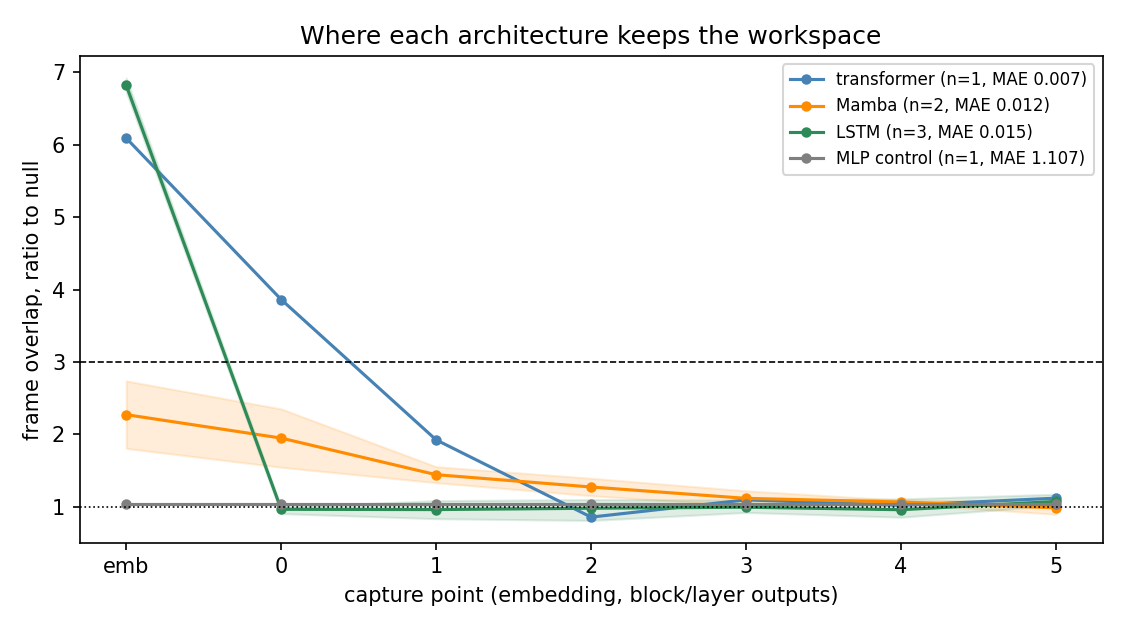
\includegraphics[width=0.72\textwidth]{figures/cross_arch_frame.png}
  \caption{\textbf{Where each architecture keeps the workspace.} Frame
  overlap (ratio to null, $r{=}8$) by capture point; bands span seeds.
  The transformer holds a frame-aligned workspace in its residual
  stream (emb--block 1); the LSTM is frame-aligned \emph{only at the
  embedding} ($6.7$--$6.9\times$, three seeds) and exactly null through
  all recurrent layers; Mamba is graded; the MLP control is null
  everywhere.}
  \label{fig:crossarch}
\end{figure}

\paragraph{The separation principle is architecture-general.} In every
calibrated architecture, the J-lens finds a causal workspace whose
contents decode the posterior's surviving set (transformer $0.998$;
LSTM $1.000$ at layer 3--4, $r{=}24$, all three seeds; Mamba $0.965$),
and in every one the entropy-readout axis is near-perfectly decodable
and causally inert (ablation $\Delta$MAE $\le 0.0002$ bits in all
three). The frame--precision dissociation is not a transformer fact; it
is a trained-Bayesian-system fact.

\paragraph{The coordinates are architecture-specific: the LSTM's
private code.} The LSTM presents a clean dissociation of its own.
Its recurrent layers sit at exactly null frame overlap, and frame
coordinates there are causally dead: projecting out the frame at hidden
layers costs nothing ($0.009 \to 0.009$ bits) and frame-component swaps
have no effect ($-6.8$ bits margin). Yet the same layers carry the full
posterior content in the LSTM's \emph{own} J-space coordinates: probes
decode the surviving set perfectly, and swapping those coordinates
between evidence-matched runs redirects the posterior by $+3.5$ to
$+4.9$ bits (three seeds). At the embedding boundary, where evidence
enters in token coordinates, the frame swap equals the full-residual
ceiling ($+6.6$ to $+6.9$ bits), after which the content is re-encoded
into a private code. Same content, same causal structure, different
coordinate system.

\paragraph{Mamba: the workspace leaves the residual stream entirely.}
On the SSM, \emph{no} positional patch redirects the posterior: not
the frame, not its own J-space, not the full residual of the entire
evidence region (best margin $-0.6$ bits). This is not
unpatchability but the wrong lever: evidence transport is distributed
through per-block scan states rather than positional residuals.
Intervening on the states themselves settles necessity robustly:
zeroing every block's state at the read boundary is catastrophic on
both seeds tested (KL to the true posterior explodes from ${\sim}0.02$
to $25$--$34$ bits; the states carry everything). Sufficiency by
transplant is not seed-stable: an evidence-matched \emph{state} swap
redirects the posterior on one seed ($+1.2$ bits at the deep read
position, halfway at mid-sequence where local convolution, skip, and
gating paths carry recent evidence) and fails on a second ($-2.3$),
plausibly because a selective SSM's donor states are
trajectory-specific in ways positional residuals are not. What stands:
the evidence lives in scan state, off the residual stream, where a
residual-stream positional lens cannot see it.

\paragraph{Reading.} The separation principle (routing substrate
versus writer computation) holds in all three architectures. What is
architecture-specific is the \emph{implementation of the routing side}:
attention keeps the substrate as a frame-aligned positional subspace of
the residual stream (its content-addressable keys require token
coordinates); the LSTM keeps the same content at layer boundaries in a
learned private code; Mamba keeps it in scan state, off the residual
stream altogether. A practical implication for production
interpretability follows: the J-lens finds workspaces where
architectures keep content in positional residual subspaces, so on
hybrid or SSM-based models the same analysis could report ``no
workspace'' while an intact, causally verified one sits in state
space. One caveat bounds the reading: this task exercises accumulation
only; on a variant requiring binding (repeated-key queries), the
recurrent architectures are expected to fail outright
\citep{agarwal2026windtunnel}, and whether their private-coordinate
substrates persist into the failure regime is an open question for the
follow-up.

\section{Discussion}

The contribution is one sentence: \emph{routing substrate is not
writer computation}. A workspace can exist, be correctly shaped, and be
causally available while the machinery that fills it is absent. The
identification results are what license this separation principle:
without P1/P3 grounding what the workspace \emph{is}, ``routing
geometry is not computation'' would be a claim about an uninterpreted
subspace. And the distinction is orthogonal to whether a workspace
exists: a model may possess an intact routing substrate yet fail to
generalize because the computations that populate it have not been
learned.

\paragraph{What is now grounded.} In this wind tunnel the \Jspace{}
is identified with the hypothesis frame (P1), it carries exactly the
posterior's support (P3), its content is what patching moves (P4), and
the formation mechanism the production paper asks for is the one already
derived for the frame: advantage-based routing builds it early, a bank
of early heads writes it, and precision arrives later (P2, dynamics).
None of this could be verified at production scale; all of it survives
verification here.

\paragraph{What changed under test.} Two preregistered predictions failed
in ways that revise the picture rather than merely bounding it. Workspace
writing is distributed but dichotomous, not concentrated. The
correct writer metric is absolute projected write, a caution that
transfers directly to the production analysis. It also bears on
low-rank adaptation: the task's functional subspace has dimension near
the hypothesis count (probes saturate once rank covers it), which is
the activation-side version of the premise LoRA rests on, and it
yields two testable corollaries. Adapters on writer layers should move
content while adapters placed late should move precision, and adapter
sites selected by relative norms are exposed to the same
anti-selection failure measured here. And the workspace does not
inherit the compilation boundary: position-bound failure lives in the
writers, now causally localized by the rescue experiment (readers are
position-general; a transplanted writer state restores post-horizon
prediction to $1.00$). In one line: \emph{workspace
existence is not workspace competence}. Stated as architecture: the
workspace is a routing substrate, and generalization depends on the
learned writers, not on the existence of the substrate itself. If this transfers to scale,
``the model has a workspace'' and ``the model can use its workspace
here'' are separate claims requiring separate evidence, a distinction
the production paper's flexibility experiments do not currently draw.

\paragraph{Relation to the independent reception.} An early independent
review of the production release~\citep{nanda2026review} replicated its
core claims on a second model family and set the practitioner's
calibration: the lens is an approximation, best treated as hypothesis
generation; expected to miss some content and to carry false positives;
and least trusted where it is used causally. The wind tunnel speaks to
all three, in both directions. On causal use: scored against the
analytic posterior, the lens-identified subspace redirects exactly as
Bayes requires (P4). On false positives: the most tempting candidate in
our setting, the perfectly decodable entropy axis, is not in the
\Jspace{} --- its projection onto the top J-directions sits at or below
the random-direction baseline at every layer (for example $0.10$ against
an expected $0.20$ at $r{=}8$, block 1) --- so the use-based definition
resists exactly the artifact that probing invites. On false negatives:
we exhibit one causally verified instance, the state-resident workspace
of \cref{sec:crossarch}, and name its mechanism. The review's implicit
missing experiment, validation on a task with known ground truth, is
this note.

\paragraph{Relation to the frame--precision dissociation.} The
separation principle has a genealogy inside this program. The
frame--precision dissociation of Papers I--III separates two kinds of
\emph{content} within a working circuit: the frame carrying posterior
support, and the precision readout riding on it, replicated causally
here by P4b (the entropy axis is perfectly decodable, $R^2 = 1.00$, and
causally inert, $-0.001$ bits). Routing-vs-computation is the same
schema one level up: not support versus confidence within content but
\emph{substrate versus process}: the coordinate system versus the
machinery that writes into it. The learning dynamics carry the same
signature at both levels: geometry first, precision second (Papers
I--II); substrate causally functional by step ${\sim}400$, writer
precision refined over the remaining 47k steps (\cref{fig:midtraining}),
with the load consolidating into frame coordinates as training
proceeds, plausibly the same EM-like sculpting described in Paper~II.
The promotion is strict: P5 exhibits the
substrate existing with the process entirely absent, a configuration
the frame--precision work had no setting to produce. The genealogy in one
sentence: frame--precision was the first cut of the separation;
the loss-horizon models supplied the setting in which the two objects
fully come apart; the J-lens supplied the instrument that measures the
substrate independently of the process.

\paragraph{Relation to identifiability theory.}
The J-lens has a formal cousin in the nonlinear-ICA identifiability
literature, which studies when latent structure is recoverable from the
Jacobian of a generative map \citep{hyvarinen1999nonlinear,
zheng2022identifiability, zheng2023generalizing, dictdiverse2026}. The
objects differ: that line proves guarantees for the Jacobian of the map
from latent sources to observations, under invertibility and structural
sparsity or diversity assumptions, while the J-lens probes the Jacobian
of a trained network's forward pass from activations to logits, where
those assumptions do not hold and no guarantee is claimed. Two of its
results nonetheless bear directly on ours. First, identifiability in
that setting holds only up to permutation and component-wise
transformation of the latents; our finding that the token-identity
frame carries the P1 overlap while head-pullback variants pass only at
low rank is recovery up to exactly such a transformation class, the
expected indeterminacy rather than a defect of the preregistration.
Second, the stated frontier of that literature is checking generalized
identifiability in trained foundation models, where ground-truth
latents are unavailable. The wind tunnel is the setting where they are
available: P1 and P3 jointly verify, in a model with an analytic
posterior, that the functional subspace the Jacobian identifies equals
the generative latent structure it should identify. To our knowledge
this is the first empirical case where the two notions can be computed
independently and compared, and they coincide.

\paragraph{The one-sentence version.} Bayesian computation factorizes
into a routing substrate and writer computation. The separation is
architecture-general; the geometric realization of the substrate is
architecture-specific. In these models, the transformer externalizes it
into a shared token frame, the LSTM internalizes it into a private
code, and the SSM moves it into scan state. That is the claim the rest
of the paper supports.

\paragraph{Limitations.} Wind-tunnel scale is the point, and the caveat:
these are 2.7M-parameter models with one in-context task each, and the
late-layer \Jspace{} is structurally degenerate for strictly-future
targets, so depth claims are confined to early/mid layers. The
identification threshold ($3\times$ null) was preregistered but the frame
mode that carries it (token-identity rather than head-pullback) was a
within-family refinement; we report all modes, and the referee controls
show the threshold is not universally met across training seeds (the
alignment magnitude is seed- and tying-dependent even though the
underlying causal structure is not). Read-connectivity ratios
here are $2$--$3.6\times$, far from the ${\sim}100\times$ reported at
production scale, consistent with a 6-layer model having little room for
specialization, but unverified. The hypothesis space is single-token by
construction, so the production-scale concern about concepts without
single-token equivalents is untested here.

\paragraph{Artifacts.} Code, per-cell grids, preregistration deviations,
and all figures: \texttt{experiments/jlens/} in the wind-tunnel
repository, pinned against \texttt{anthropics/jacobian-lens}
\texttt{@581d3986}. The full study is reproducible in ${\sim}2$ GPU-hours
on one consumer GPU.

\bibliographystyle{plainnat}
\bibliography{references}

\end{document}
